\documentclass[tikz,border=14pt]{standalone}
\usepackage{xcolor}
\usepackage{tikz}
\usetikzlibrary{arrows.meta, positioning, fit, backgrounds, calc, shapes.geometric}

\usepackage{fontspec}

% --- Anthropic Color Tokens ---
\definecolor{bgWarm}{HTML}{FAF8F3}
\definecolor{bgPanel}{HTML}{FFFDFC}
\definecolor{laneStroke}{HTML}{D7D0C5}
\definecolor{connectorStroke}{HTML}{9EA9B1}
\definecolor{inkText}{HTML}{31424B}
\definecolor{mutedText}{HTML}{66757E}

\definecolor{lavFill}{HTML}{E7E3FF}
\definecolor{lavStroke}{HTML}{8D86D8}
\definecolor{lavText}{HTML}{373457}
\definecolor{lavSubtext}{HTML}{5852A7}

\definecolor{mintFill}{HTML}{DDF4EC}
\definecolor{mintStroke}{HTML}{78B5A7}
\definecolor{mintText}{HTML}{294B45}
\definecolor{mintSubtext}{HTML}{3F8F7F}

\definecolor{tealFill}{HTML}{D9F0F2}
\definecolor{tealStroke}{HTML}{6CA9B0}
\definecolor{tealText}{HTML}{29464A}
\definecolor{tealSubtext}{HTML}{457E85}

\definecolor{creamFill}{HTML}{F4EEE3}
\definecolor{creamStroke}{HTML}{C1B39E}
\definecolor{creamText}{HTML}{4E4437}
\definecolor{creamSubtext}{HTML}{8E7A61}

\definecolor{amberFill}{HTML}{F8E7C9}
\definecolor{amberStroke}{HTML}{D6A86B}
\definecolor{amberText}{HTML}{57401C}
\definecolor{amberSubtext}{HTML}{A27431}

\definecolor{peachFill}{HTML}{F8E0D9}
\definecolor{peachStroke}{HTML}{CF8E81}
\definecolor{peachText}{HTML}{55342E}
\definecolor{peachSubtext}{HTML}{A66559}

\pagecolor{bgWarm}

\newcommand{\anthropicLabel}[4]{%
  \def\tmp{#4}%
  \ifx\tmp\empty
    {\sffamily\bfseries\small\textcolor{#1}{#3}}%
  \else
    \begin{tabular}{@{}c@{}}
      {\sffamily\bfseries\small\textcolor{#1}{#3}}\\[-1pt]
      {\sffamily\fontsize{8}{9}\selectfont\textcolor{#2}{#4}}
    \end{tabular}%
  \fi
}

\begin{document}

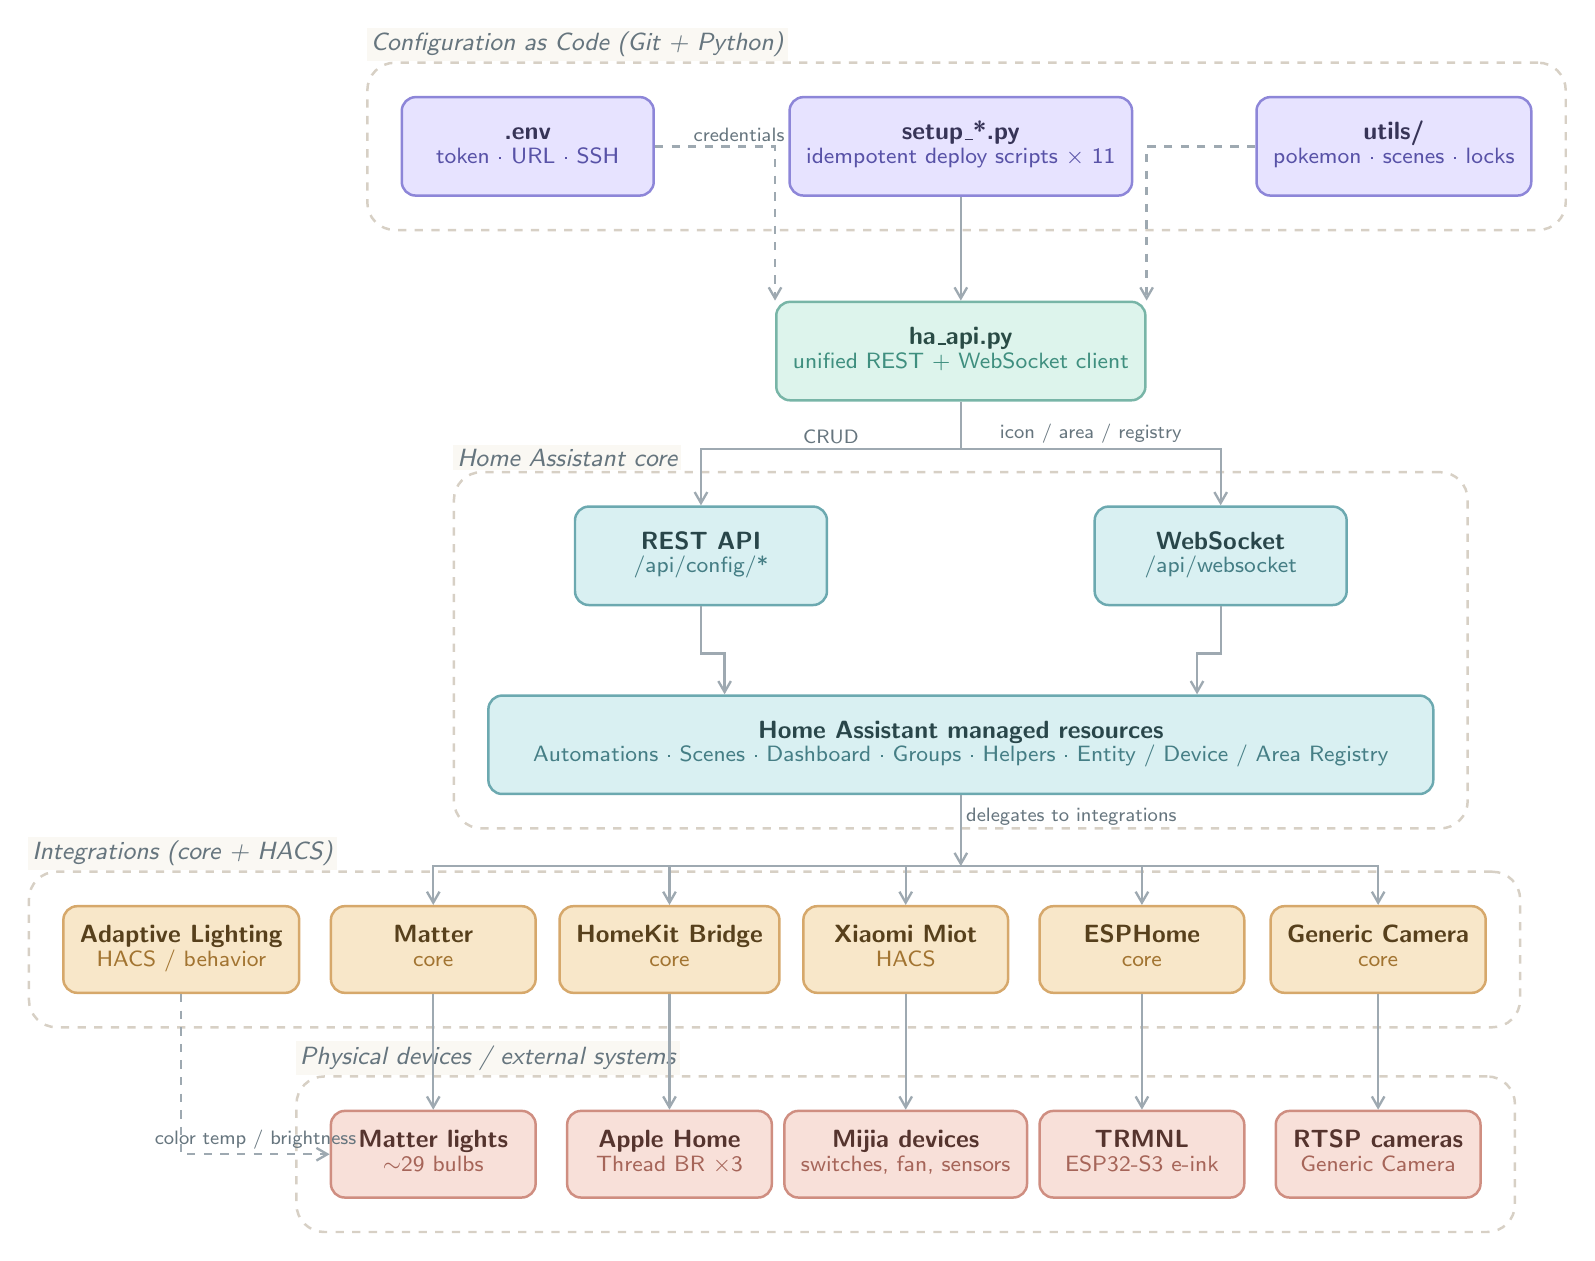
\begin{tikzpicture}[
    x=1cm,
    y=1cm,
    font=\sffamily\footnotesize,
    anthropicEdge/.style={
        -{Straight Barb[angle=60:2pt 3]},
        draw=connectorStroke,
        line width=0.85pt
    },
    anthropicDashedEdge/.style={
        anthropicEdge,
        dashed
    },
    anthropicCardNode/.style={
        rectangle,
        rounded corners=5pt,
        draw,
        line width=0.9pt,
        minimum width=3.2cm,
        minimum height=1.25cm,
        inner sep=6pt,
        align=center,
        fill=bgPanel
    },
    anthropicSmallCard/.style={
        anthropicCardNode,
        minimum width=2.6cm,
        minimum height=1.1cm
    },
    anthropicWideCard/.style={
        anthropicCardNode,
        minimum width=12cm,
        minimum height=1.25cm
    },
    anthropicGroup/.style={
        rectangle,
        rounded corners=10pt,
        draw=laneStroke,
        dashed,
        line width=0.9pt,
        inner sep=12pt,
        fill opacity=0
    },
    anthropicGroupTitle/.style={
        font=\sffamily\itshape\small,
        text=mutedText,
        fill=bgWarm,
        inner sep=1.5pt
    },
    edgeLabel/.style={
        font=\sffamily\scriptsize,
        text=mutedText,
        fill=none,
        inner sep=1.5pt,
        align=center
    }
]

    % --- Tier 1: Configuration as Code ---
    \node[anthropicCardNode, draw=lavStroke, fill=lavFill] (env) at (0,0)
        {\anthropicLabel{lavText}{lavSubtext}{.env}{token \textperiodcentered\ URL \textperiodcentered\ SSH}};
    \node[anthropicCardNode, draw=lavStroke, fill=lavFill, minimum width=4cm] (scripts) at (5.5,0)
        {\anthropicLabel{lavText}{lavSubtext}{setup\_*.py}{idempotent deploy scripts $\times$ 11}};
    \node[anthropicCardNode, draw=lavStroke, fill=lavFill] (utils) at (11,0)
        {\anthropicLabel{lavText}{lavSubtext}{utils/}{pokemon \textperiodcentered\ scenes \textperiodcentered\ locks}};

    % --- Tier 2: API layer ---
    \node[anthropicCardNode, draw=mintStroke, fill=mintFill, minimum width=4.2cm] (api) at (5.5,-2.6)
        {\anthropicLabel{mintText}{mintSubtext}{ha\_api.py}{unified REST + WebSocket client}};

    % --- Tier 3: HA Core APIs ---
    \node[anthropicCardNode, draw=tealStroke, fill=tealFill] (rest) at (2.2,-5.2)
        {\anthropicLabel{tealText}{tealSubtext}{REST API}{/api/config/*}};
    \node[anthropicCardNode, draw=tealStroke, fill=tealFill] (ws) at (8.8,-5.2)
        {\anthropicLabel{tealText}{tealSubtext}{WebSocket}{/api/websocket}};

    % --- Tier 4: HA managed resources ---
    \node[anthropicWideCard, draw=tealStroke, fill=tealFill] (resources) at (5.5,-7.6)
        {\anthropicLabel{tealText}{tealSubtext}{Home Assistant managed resources}{Automations \textperiodcentered\ Scenes \textperiodcentered\ Dashboard \textperiodcentered\ Groups \textperiodcentered\ Helpers \textperiodcentered\ Entity / Device / Area Registry}};

    % --- Tier 5: Integrations ---
    \node[anthropicSmallCard, draw=amberStroke, fill=amberFill] (matter) at (-1.2,-10.2)
        {\anthropicLabel{amberText}{amberSubtext}{Matter}{core}};
    \node[anthropicSmallCard, draw=amberStroke, fill=amberFill] (homekit) at (1.8,-10.2)
        {\anthropicLabel{amberText}{amberSubtext}{HomeKit Bridge}{core}};
    \node[anthropicSmallCard, draw=amberStroke, fill=amberFill] (xiaomi) at (4.8,-10.2)
        {\anthropicLabel{amberText}{amberSubtext}{Xiaomi Miot}{HACS}};
    \node[anthropicSmallCard, draw=amberStroke, fill=amberFill] (esphome) at (7.8,-10.2)
        {\anthropicLabel{amberText}{amberSubtext}{ESPHome}{core}};
    \node[anthropicSmallCard, draw=amberStroke, fill=amberFill] (genericcam) at (10.8,-10.2)
        {\anthropicLabel{amberText}{amberSubtext}{Generic Camera}{core}};

    % Behavioral side-integration (no physical device of its own)
    \node[anthropicSmallCard, draw=amberStroke, fill=amberFill] (adaptive) at (-4.4,-10.2)
        {\anthropicLabel{amberText}{amberSubtext}{Adaptive Lighting}{HACS / behavior}};

    % --- Tier 6: Physical devices ---
    \node[anthropicSmallCard, draw=peachStroke, fill=peachFill] (lights) at (-1.2,-12.8)
        {\anthropicLabel{peachText}{peachSubtext}{Matter lights}{$\sim$29 bulbs}};
    \node[anthropicSmallCard, draw=peachStroke, fill=peachFill] (threadbr) at (1.8,-12.8)
        {\anthropicLabel{peachText}{peachSubtext}{Apple Home}{Thread BR $\times$3}};
    \node[anthropicSmallCard, draw=peachStroke, fill=peachFill] (miji) at (4.8,-12.8)
        {\anthropicLabel{peachText}{peachSubtext}{Mijia devices}{switches, fan, sensors}};
    \node[anthropicSmallCard, draw=peachStroke, fill=peachFill] (trmnl) at (7.8,-12.8)
        {\anthropicLabel{peachText}{peachSubtext}{TRMNL}{ESP32-S3 e-ink}};
    \node[anthropicSmallCard, draw=peachStroke, fill=peachFill] (cams) at (10.8,-12.8)
        {\anthropicLabel{peachText}{peachSubtext}{RTSP cameras}{Generic Camera}};

    % --- Connectors: Tier 1 -> Tier 2 ---
    \draw[anthropicEdge] (scripts.south) -- (api.north);
    \draw[anthropicDashedEdge] (env.east) -| node[pos=0.35, edgeLabel, above] {credentials} (api.north west);
    \draw[anthropicDashedEdge] (utils.west) -| (api.north east);

    % --- Connectors: Tier 2 -> Tier 3 ---
    \coordinate (apiSplit) at ($(api.south)+(0,-0.6)$);
    \draw[anthropicEdge, -] (api.south) -- (apiSplit);
    \draw[anthropicEdge] (apiSplit) -| node[pos=0.25, edgeLabel, above] {CRUD} (rest.north);
    \draw[anthropicEdge] (apiSplit) -| node[pos=0.25, edgeLabel, above] {icon / area / registry} (ws.north);

    % --- Connectors: Tier 3 -> Tier 4 ---
    \draw[anthropicEdge] (rest.south) -- ($(rest.south)+(0,-0.6)$) -| ($(resources.north)+(-3,0)$);
    \draw[anthropicEdge] (ws.south) -- ($(ws.south)+(0,-0.6)$) -| ($(resources.north)+(3,0)$);

    % --- Connectors: Tier 4 -> Tier 5 (fan out to integrations) ---
    \draw[anthropicEdge] (resources.south) -- ++(0,-0.9)
        node[edgeLabel, above right, pos=0.5] {delegates to integrations}
        coordinate (bus);
    \draw[anthropicEdge] (bus) -| (matter.north);
    \draw[anthropicEdge] (bus) -| (homekit.north);
    \draw[anthropicEdge] (bus) -| (xiaomi.north);
    \draw[anthropicEdge] (bus) -| (esphome.north);
    \draw[anthropicEdge] (bus) -| (genericcam.north);

    % --- Connectors: Tier 5 -> Tier 6 (1:1 vertical) ---
    \draw[anthropicEdge] (matter.south) -- (lights.north);
    \draw[anthropicEdge] (homekit.south) -- (threadbr.north);
    \draw[anthropicEdge] (xiaomi.south) -- (miji.north);
    \draw[anthropicEdge] (esphome.south) -- (trmnl.north);
    \draw[anthropicEdge] (genericcam.south) -- (cams.north);

    % Adaptive Lighting is a behavioral integration on top of existing Matter lights
    \draw[anthropicDashedEdge] (adaptive.south) |- node[edgeLabel, above, pos=0.75] {color temp / brightness} (lights.west);

    % --- Groups ---
    \begin{scope}[on background layer]
        \node[
            anthropicGroup,
            fit=(env) (scripts) (utils),
            label={[anthropicGroupTitle, anchor=south west]north west:{Configuration as Code (Git + Python)}}
        ] {};
        \node[
            anthropicGroup,
            fit=(rest) (ws) (resources),
            label={[anthropicGroupTitle, anchor=south west]north west:{Home Assistant core}}
        ] {};
        \node[
            anthropicGroup,
            fit=(adaptive) (matter) (homekit) (xiaomi) (esphome) (genericcam),
            label={[anthropicGroupTitle, anchor=south west]north west:{Integrations (core + HACS)}}
        ] {};
        \node[
            anthropicGroup,
            fit=(lights) (threadbr) (miji) (trmnl) (cams),
            label={[anthropicGroupTitle, anchor=south west]north west:{Physical devices / external systems}}
        ] {};
    \end{scope}

\end{tikzpicture}
\end{document}
